% !TEX encoding = UTF-8 Unicode
\section{ScaLAPACK - Scalable Linear Algebra PACKage}
%%%%%%%%%%%%%%%%
	\begin{frame}{ScaLAPACK - Scalable Linear Algebra PACKage}
		1991 - 1994 (Feb. 1995) \\
		LAPACK-DM - multicomputers, MIMD \\
		\vspace{5mm}
		BLACS - Basic Linear Algebra Communication Subprogramme \\
		BLAS \\
		PBLAS \\
		\vspace{5mm}
		(Jack Dongarra - PVM, MPI)
		\vspace{5mm}

	\end{frame}
	\begin{frame}{ScaLAPACK - Scalable Linear Algebra PACKage}
		\begin{figure}
			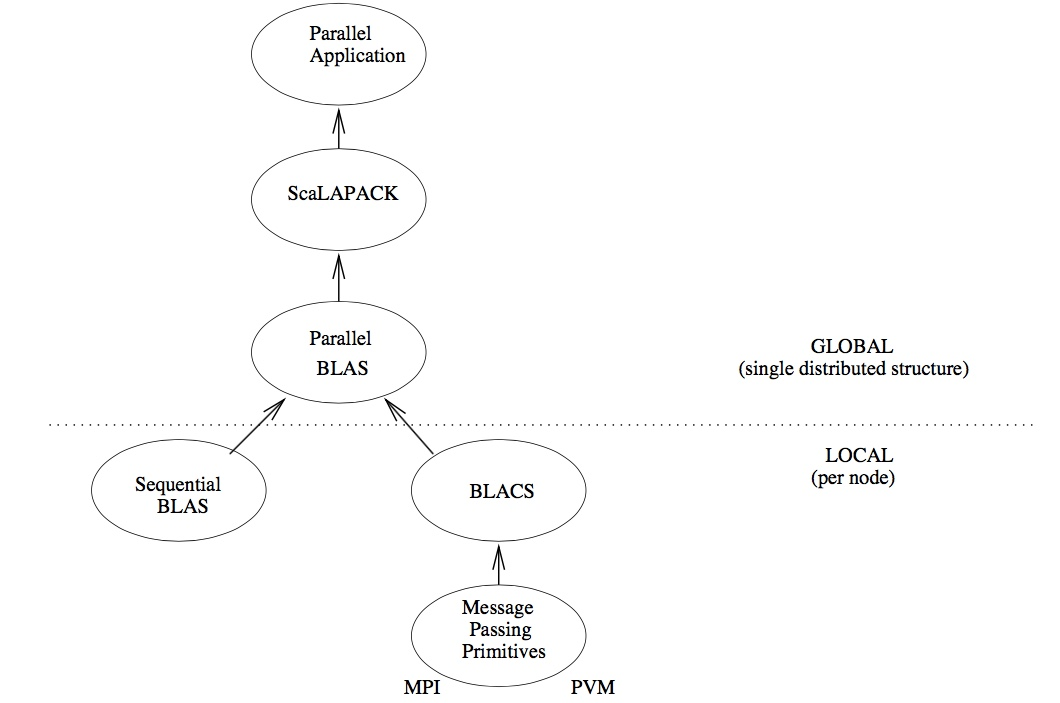
\includegraphics[height=7cm]{img/13/scalapack}
		\end{figure}
	\end{frame}
	\begin{frame}{BLACS - the Basic Linear Algebra Communication Subprograms}
		Operacje: 
		\begin{itemize}
			\item	\textbf{send/recv} - przesyłanie (pod)macierzy z jednego procesu do drugiego
			\item \textbf{broadcast} - przesyłanie (pod)macierzy do wszystkich procesów lub do podzbioru procesów wg określonego sposobu
			\item \textbf{global combine operations} - czyli: SUM, $|MIN|$, $|MAX|$, wykonywanie operacji na określonej macierzy
		\end{itemize}
		Procesy na siatce 2-D:
		\begin{tabular}{ c|c|c|c|c| }
			\multicolumn{1}{c}{} & \multicolumn{1}{c}{0} & \multicolumn{1}{c}{1} & \multicolumn{1}{c}{2} & \multicolumn{1}{c}{3} \\
			\cline{2-5} 0 & 0 & 1 & 2 & 3 \\
			\cline{2-5} 1 & 4 & 5 & 6 & 7 \\
			\cline{2-5} 2 & 8 & 9 & 10 & 11 \\
			\cline{2-5}
		\end{tabular} \\
		Na przykład: xxSD2D(icontxt, m, n, a, lda, rdest, cdest)
	\end{frame}
	
	\begin{frame}{PBLAS - the Parallel Basic Linear Algebra Subprograms for distributed memory MIMD computers}
		\begin{itemize}
			\item Funkcjonalność - jak BLAS: distributed vector-vector, vector-matrix, matrix-matrix operations,
			\item Uproszczenie zrównoleglenia,
			\item Przejrzystość,
			\item Modularność,
			\item Przenośność,
			\item SPDM programming model.
		\end{itemize}
		Sposób przechowywania macierzy:
		\begin{tabular}{ l l | l l | l }
		$a_{11}$ & $a_{12}$ & $a_{13}$ & $a_{14}$ & $a_{15}$ \\
		$a_{21}$ & $a_{22}$ & $a_{23}$ & $a_{24}$ & $a_{25}$ \\
		\hline
		$a_{31}$ & $a_{32}$ & $a_{33}$ & $a_{34}$ & $a_{35}$ \\
		$a_{41}$ & $a_{42}$ & $a_{43}$ & $a_{44}$ & $a_{45}$ \\
		\hline
		$a_{51}$ & $a_{52}$ & $a_{53}$ & $a_{54}$ & $a_{55}$ \\
		\end{tabular}
	\end{frame}
	\begin{frame}{PBLAS - the Parallel Basic Linear Algebra Subprograms for distributed memory MIMD computers}
		\begin{tabular}{ c | c c c | c c | }
			\multicolumn{1}{c}{} & \multicolumn{1}{c}{0} & \multicolumn{1}{c}{} & \multicolumn{1}{c}{} & \multicolumn{1}{c}{1} \\
		\cline{2-6} & $a_{11}$ & $a_{12}$ & $a_{15}$ & $a_{13}$ & $a_{14}$ \\
		0 & $a_{21}$ & $a_{22}$ & $a_{25}$ & $a_{23}$ & $a_{24}$ \\
		 & $a_{51}$ & $a_{52}$ & $a_{55}$ & $a_{53}$ & $a_{54}$ \\
	
		\cline{2-6} & $a_{31}$ & $a_{32}$ & $a_{35}$ & $a_{33}$ & $a_{34}$ \\
		1& $a_{41}$ & $a_{42}$ & $a_{45}$ & $a_{43}$ & $a_{44}$ \\
		\cline{2-6}
		
		\end{tabular} \\
		\vspace{5mm}
		5x5  macierz $\rightarrow$ bloki 2x2 $\Rightarrow$ na 2x2 siatce procesów \\
		2-dimensional block-cycling scheme $\Rightarrow$ \\
		\begin{itemize}
			\item load-balance
			\item scalability
		\end{itemize}
	\end{frame}
	
	\begin{frame}{Object oriented extensions of ScaLAPACK}
		\begin{itemize}
			\item użytkownicy
			\item możliwość enkapsulacji
		\end{itemize}
		\begin{figure}
			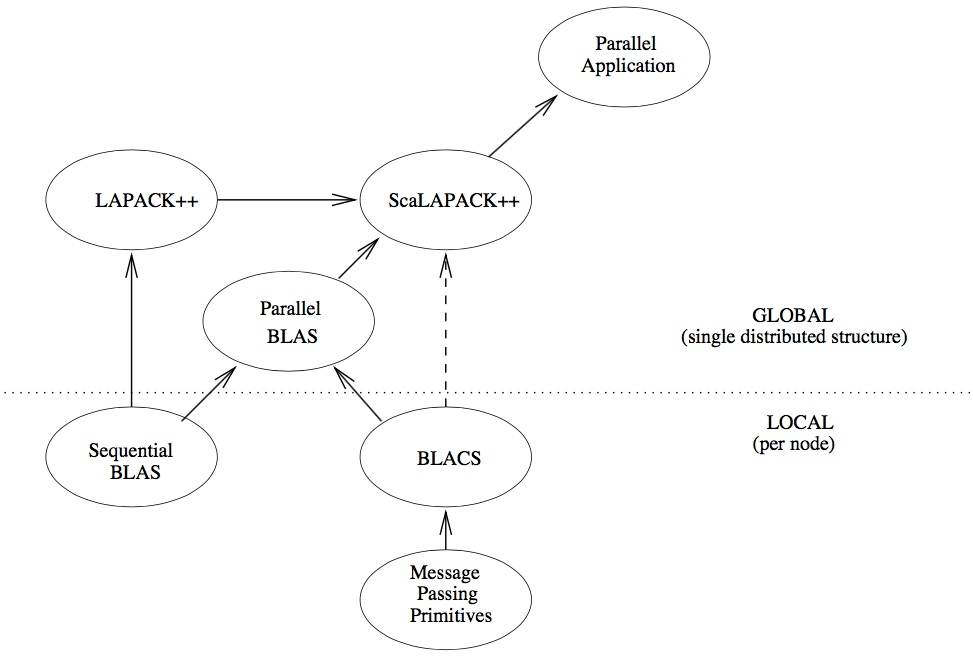
\includegraphics[height=6cm]{img/13/scalapackextensions}
		\end{figure}
	\end{frame}